\documentclass{beamer}
\beamertemplatenavigationsymbolsempty
\usepackage[french]{babel}
\usepackage{fontspec}
\usepackage{amsmath, amsthm, amsfonts}
\usepackage[separate-uncertainty]{siunitx}
\usepackage{xcolor}
\usepackage{tikz}
\usepackage{tikz-cd}
\usepackage[object=vectorian]{pgfornament}
\usepackage{circuitikz}
\usepackage{hyperref}
\usepackage{caption}
\usepackage{booktabs}
\usepackage{mathtools}
\usepackage{longtable}
\usepackage[version=3]{mhchem}
\usepackage{marginnote}
\usepackage[framemethod=tikz]{mdframed}


% Paul Tol's qualitative palette
% ``bright''.https://personal.sron.nl/~pault/#sec:qualitative
\definecolor{tblue}{HTML}{4477AA}
\definecolor{tcyan}{HTML}{66CCEE}
\definecolor{tgreen}{HTML}{228833}
\definecolor{tyellow}{HTML}{CCBB44}
\definecolor{tred}{HTML}{EE6677}
\definecolor{tpurple}{HTML}{AA3377}
\definecolor{tgrey}{HTML}{BBBBBB}


% Justification for marginnotes.
\renewcommand*{\raggedleftmarginnote}{}
\renewcommand*{\raggedrightmarginnote}{}


% Styles for mdframed environments.
\newmdenv[backgroundcolor=tgreen!10,linecolor=tgreen!30]{reponsebox}
\newmdenv[backgroundcolor=tyellow!10,linecolor=tyellow!30]{diapobox}
\newmdenv[backgroundcolor=tred!10,linecolor=tred!30]{fondamentalbox}

% Default arrow for tikz and style for positive and negative objects.
\tikzset{>=latex,
    negative/.style={draw=teal!70!black, fill=teal!10, thick},
    positive/.style={draw=red, fill=red!10, thick}}
\usetikzlibrary{matrix,calc,decorations.pathreplacing,decorations.pathmorphing,decorations.markings}

% French locale for numbers and negative exponent for units.
\sisetup{locale=FR, per-mode=symbol}

\newcommand{\abs}[1]{\left| #1 \right|}
\newcommand{\rhat}{\vec{\hat{r}}}
\newcommand{\xhat}{\vec{\imath}}
\newcommand{\yhat}{\vec{\jmath}}
\newcommand{\zhat}{\vec{k}}
\newcommand{\real}{\mathbb{R}}
\newcommand{\der}[2]{\frac{\mathrm{d}#1}{\mathrm{d}#2}}
\newcommand{\pder}[2]{\frac{\partial\ #1}{\partial\ #2}}
\newcommand{\dif}{\mathrm{d}}
\newcommand{\ddif}{\,\mathrm{d}}
\newcommand{\grad}{\vec{\nabla}}
\newcommand{\exemple}[1]{\begin{fullwidth}#1\end{fullwidth}}
\newcommand{\norm}[1]{\lVert\ #1\ \rVert}
\newcommand{\vu}{\vec{u}}
\newcommand{\vv}{\vec{v}}
\newcommand{\vr}{\vec{r}}
\newcommand{\va}{\vec{a}}
\newcommand{\vF}{\vec{F}}
\newcommand{\vE}{\vec{E}}
\newcommand{\vB}{\vec{B}}
\newcommand{\vecxyz}[3]{#1 \xhat\ + #2 \yhat\ + #3 \zhat}
\newcommand{\vecxy}[2]{#1 \xhat\ + #2 \yhat}
\newcommand{\coulombcst}{k}
\newcommand{\emf}{\ensuremath{\mathcal{E}}}
\newcommand{\eval}{\SI{1.602e-19}{C}}
\newcommand{\kval}{\SI{8.99e9}{Nm^2 \per C^2}}

% Nice separator line
\newcommand{\sectionline}{
    \noindent
    \begin{center}
        \resizebox{0.5\linewidth}{1ex}
    {{%
    {\begin{tikzpicture}
    \node  (C) at (0,0) {};
    \node (D) at (9,0) {};
    \path (C) to [ornament=85] (D);
    \end{tikzpicture}}}}
    \end{center}
}

\theoremstyle{definition}
\newtheorem*{defn}{Definition}


\usepackage[version=3]{mhchem}

\setbeamercolor{title}{fg=tblue}
\setbeamercolor{frametitle}{fg=tblue}
\setbeamercolor{structure}{fg=tblue}

% Make footnotesize smaller
\makeatletter
\renewcommand\footnotesize{%
   \@setfontsize\footnotesize\@viipt{11}%
   \abovedisplayskip 8\p@ \@plus2\p@ \@minus4\p@
   \abovedisplayshortskip \z@ \@plus\p@
   \belowdisplayshortskip 4\p@ \@plus2\p@ \@minus2\p@
   \def\@listi{\leftmargin\leftmargini
               \topsep 4\p@ \@plus2\p@ \@minus2\p@
               \parsep 2\p@ \@plus\p@ \@minus\p@
               \itemsep \parsep}%
   \belowdisplayskip \abovedisplayskip
}
\makeatother

\title{Électricité et magnétisme}
\subtitle{Chapitre 3 - Théorème de Gauss}
\date{13 septembre 2021}
\author{Loïc Séguin-Charbonneau}
\institute{Cégep Édouard-Montpetit}


\begin{document}

\maketitle


\begin{frame}[t]{Objet conducteur dans un champ uniforme}
  On place un objet métallique entre deux grandes plaques chargées
  uniformément.

  Laquelle des images ci-dessous montre
  la \textbf{séparation de charges induite} dans l'objet métallique?

  \begin{center}
    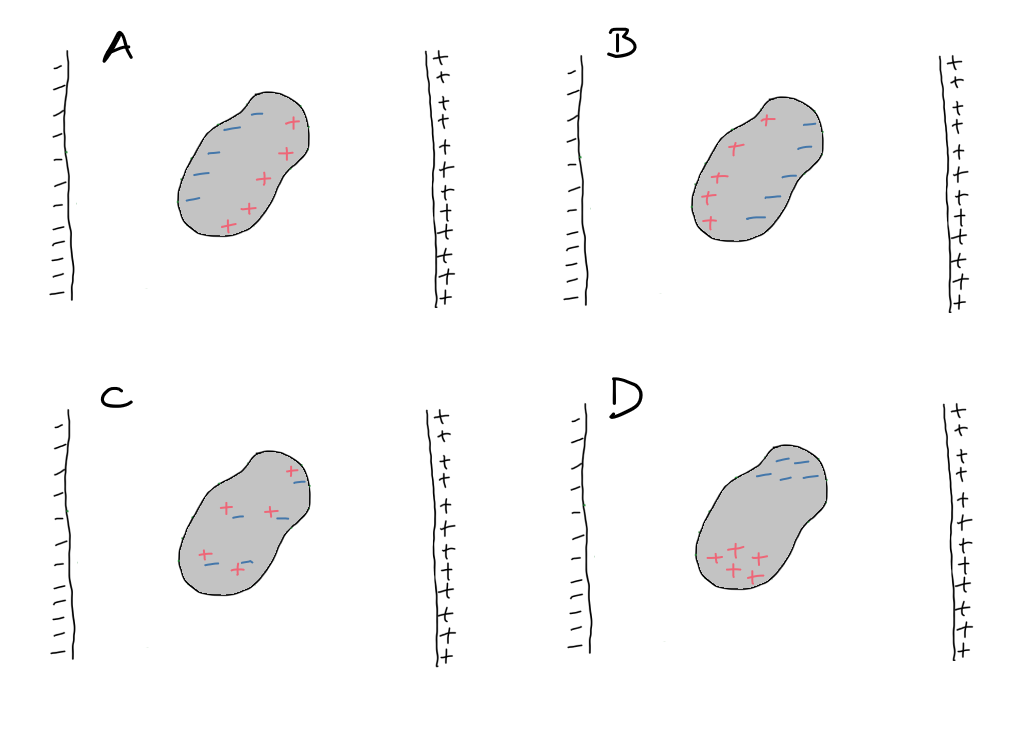
\includegraphics[width=0.9\textwidth]{figures/champ_uniforme_charges_induites.png}
  \end{center}

\end{frame}


\begin{frame}[t]{Objet conducteur dans un champ uniforme}
  On place un objet métallique entre deux grandes plaques chargées
  uniformément.

  Laquelle des images ci-dessous montre
  le champ électrique produit par les \textbf{grandes plaques} seulement?


  \begin{center}
    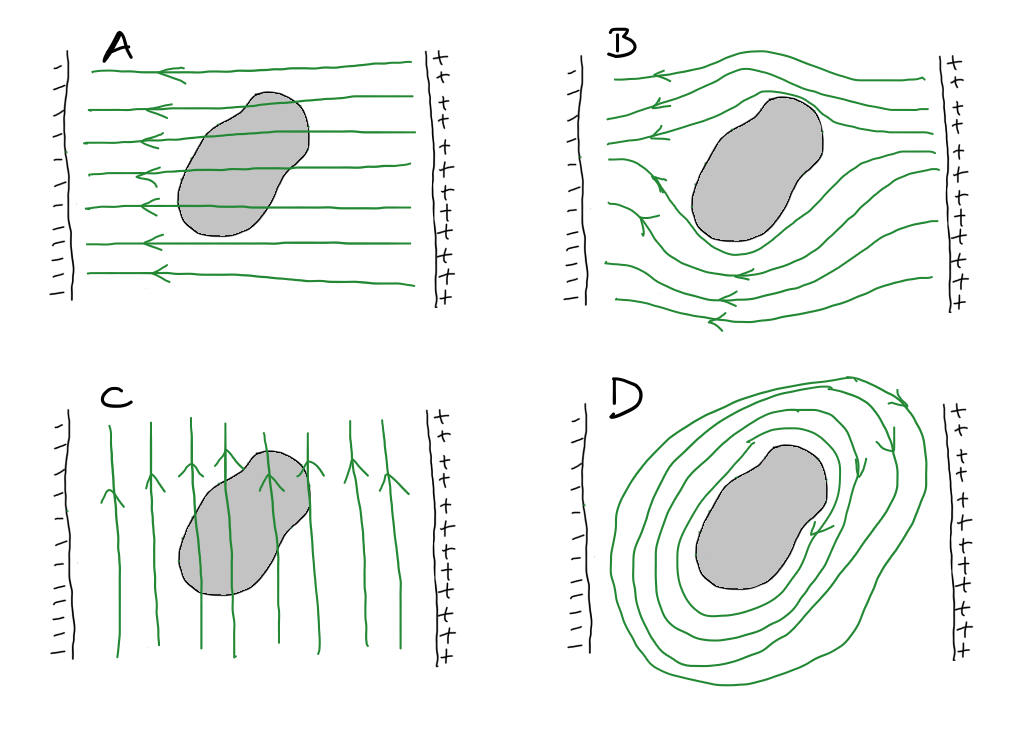
\includegraphics[width=0.9\textwidth]{figures/champ_uniforme_champ_plaque.png}
  \end{center}
\end{frame}


\begin{frame}[t]{Objet conducteur dans un champ uniforme}
  On place un objet métallique entre deux grandes plaques chargées
  uniformément.

  Laquelle des images ci-dessous montre
  le champ électrique produit par les \textbf{charges induites de l'objet
    métallique} seulement?


  \begin{center}
    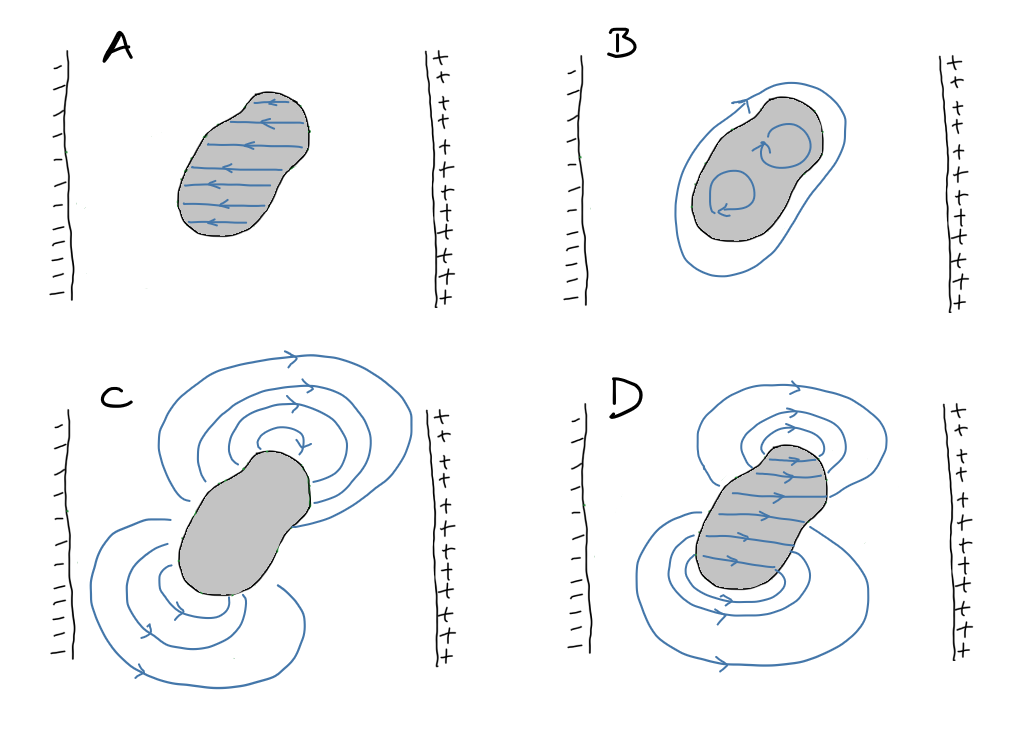
\includegraphics[width=0.9\textwidth]{figures/champ_uniforme_champ_blob.png}
  \end{center}
\end{frame}


\begin{frame}[t]{Objet conducteur dans un champ uniforme}
  On place un objet métallique entre deux grandes plaques chargées
  uniformément.

  Laquelle des images ci-dessous montre
  le champ électrique \textbf{total}?
  \vspace{\baselineskip}


  \begin{center}
    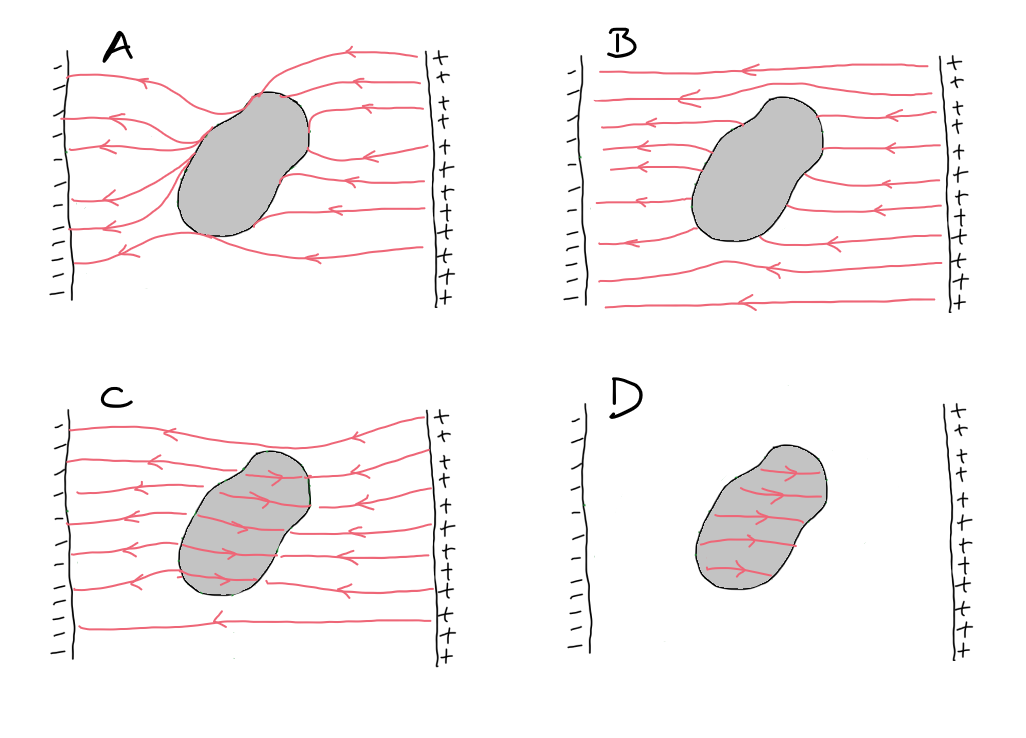
\includegraphics[width=0.9\textwidth]{figures/champ_uniforme_champ_net.png}
  \end{center}
\end{frame}



\begin{frame}[t]{Cage de Faraday}
  Gontran s'enferme dans une cage en métal pour bloquer les ondes radios en
  provenance d'une antenne à proximité.

  \onslide<3>{
    À un certain moment, le champ électrique autour de Gontran et sa cage
    pointe vers le haut. Comment sont réparties les charges électriques dans le
    matériel qui compose la cage de Gontran à ce moment? Quel est le champ
    électrique à l'intérieur de la cage?
  }

  \begin{center}
    \includegraphics<1>[width=0.9\textwidth]{figures/faraday_0.png}

    \includegraphics<2>[width=0.9\textwidth]{figures/faraday_1.png}

    \includegraphics<3>[width=0.9\textwidth]{figures/faraday_2.png}
  \end{center}
\end{frame}


\begin{frame}{Charge dans une cage de Faraday}
  Gontran a amené une charge négative de \SI{-10}{\micro\coulomb} dans sa cage de Faraday.

  \only<1>{
    Comment sont réparties les charges dans la cage? Esquissez les lignes de
    champ.
  }

  \only<2>{
    Tamara est à l'extérieur de la cage, peut-elle savoir que Gontran a une
    charge négative sans regarder à l'intérieur?
  }

  \begin{center}
    \includegraphics<1>[width=0.9\textwidth]{figures/gontran_charge.png}

    \includegraphics<2>[width=0.9\textwidth]{figures/gontran_charge_tamara.png}
  \end{center}
\end{frame}

\end{document}
